\chapter{Аналитический раздел}

\section{Общие сведения о построении изображений}

Основным устройством для получения изображений является камера, среди которых выделяются две категории: пленочные и цифровые. 

В пленочных камерах для получения изображений используется пленка. Пленка представляет собой полосу светочувствительного материала, который подвергается воздействию света при съемке. Когда пленка проявляется, экспонированные участки преобразуются в видимое изображение. Пленочные фотоаппараты распространены меньше, чем цифровые, но некоторые фотографы все еще предпочитают их за уникальный внешний вид и творческие возможности \cite{filmcameras}.

Цифровые камеры используют датчик изображения для улавливания света и преобразования его в цифровой вид. Датчик изображения представляет собой микросхему, содержащую миллионы крошечных светочувствительных транзисторов, называемых фотодиодами. Когда свет попадает на фотодиод, он генерирует электрический заряд, который пропорционален интенсивности света.

Датчик изображения представляет собой сетку пикселей, каждый из которых соответствует одному фотодиоду. Интенсивность света, падающего на каждый пиксель, записывается в виде цифрового значения, называемого значением пикселя. Совокупность значений пикселей для всех пикселей датчика изображения называется цифровым изображением.

Цифровые камеры включают в себя объектив, который фокусирует свет от сцены на датчик изображения. Диафрагма объектива описывает количество света, попадающего в камеру, а затвор --- время, в течение которого датчик изображения подвергается воздействию света.

Помимо датчика изображения и объектива, цифровые фотоаппараты оснащены электроникой, которая управляет такими функциями фотоаппарата, как фокусировка, баланс белого и обработка изображения \cite{digitalcameras}.

Цифровые камеры обладают рядом преимуществ по сравнению с пленочными \cite{fvsdcameras}:

\begin{itemize}
    \item \textit{Удобство}. Цифровые камеры позволяют просматривать и редактировать снимки сразу после съемки, т.е. не нужно ждать, пока пленка будет проявлена, чтобы увидеть результаты съемки.
    \item \textit{Хранение и совместное использование}. Цифровые камеры позволяют хранить снимки на карте памяти или компьютере и легко делиться ими по электронной почте, в социальных сетях или на других цифровых платформах. При использовании пленочных фотоаппаратов необходимо проявить и распечатать пленку, прежде чем можно будет просмотреть или поделиться снимками.
    \item \textit{Стоимость}. Использование цифровых камер обычно обходится дешевле, чем пленочных, поскольку отсутствует необходимость покупать пленку или платить за ее обработку.
    \item \textit{Универсальность}. Цифровые камеры позволяют настраивать экспозицию, баланс белого и другие параметры изображения после того, как оно было снято. В пленочных фотоаппаратах необходимо правильно настроить экспозицию и другие параметры во время съемки, поскольку после этого их нельзя отрегулировать.
    \item \textit{Качество}. Современные цифровые камеры способны создавать высококачественные изображения с широким динамическим диапазоном и точными цветами.
    \item \textit{Скорость}. Цифровые камеры, как правило, быстрее пленочных, поскольку они могут делать несколько снимков подряд. Это полезно при съемке быстро движущихся объектов или для того, чтобы сделать несколько снимков для увеличения шансов получить хорошее изображение.
\end{itemize}

Ввиду различных физических процессов на изображениях возникают помехи и ухудшают визуальное восприятие. Помехами на изображениях называют случайное изменение яркости или цвета произвольного пикселя, которое может быть вызвано несколькими факторами. Шум изображения можно увидеть в виде зернистого или крапчатого рисунка на изображении, и он может быть особенно заметен в областях с однородным цветом или слабым освещением \cite{basicnoise}.

С физической точки зрения шумы на изображениях могут возникать по следующим причинам\cite{noisephysics}:

\begin{itemize}
    \item \textit{Тепловой шум}. Тепловой шум вызван случайным движением электронов внутри датчика изображения. При повышении температуры датчика изображения движение электронов усиливается, что приводит к увеличению теплового шума.
    \item \textit{Квантовый шум}. Квантовый шум вызван случайностью квантово-механических процессов, происходящих в датчике изображения. Этот шум присущ датчику изображения и присутствует даже при низком уровне освещенности.
    \item \textit{Шум считывания}. Шум считывания вызван электрическим шумом, вносимым схемой, которая считывает данные изображения с датчика изображения. Этот шум чаще возникает при высоких значениях светочувствительности, так как схема вынуждена усиливать сигнал с датчика изображения.
\end{itemize}

В общем виде шумы некоторого изображения могут быть описаны следующим образом:
\begin{equation}
    Y = X + N,
\end{equation}
где $Y$ --- изображение с помехами, $X$ --- истинное изображение, $N$ --- шум. 

\section{Виды помех на изображениях}

Существует несколько типов шумов, которые могут возникать на изображении.

\textit{\textbf{Гауссовский шум}}. Гауссовский шум --- тип шума, который часто встречается в системах обработки сигналов и связи. Это тип статистического шума, который характеризуется функцией плотности вероятности, которая следует гауссовскому распределению, также известному как нормальное \cite{noisetypes}.

В математических терминах гауссовский шум может быть описан следующей функцией плотности вероятности:

\begin{equation}
    f(x) = \frac{1}{\sqrt{2 \pi \sigma^2}} \exp \left( -\frac{(x - \mu)^2}{2 \sigma^2} \right),
\end{equation}
где
\begin{itemize}
    \item $f(x)$ --- функция плотности вероятности шума;
    \item $x$ --- значение шума;
    \item $\mu$ --- среднее значение шума, также известное как ожидаемое значение или среднее значение;
    \item $\sigma^2$ --- дисперсия шума, которая определяет разброс распределения шума вокруг среднего значения.
\end{itemize}

Гауссов шум часто встречается в электронных системах, например, в цифровых изображениях или аудио сигналах, где он может быть вызван различными источниками, такими как тепловой шум и электронные помехи. Он также часто используется в качестве модели статистического шума в различных приложениях, таких как обработка изображений и системы связи.

На рисунке \ref{fig:gaussian_noise} представлен пример шума Гаусса.

\begin{figure}[h!]
  \centering
  \begin{tabular}{cc}
    \begin{subfigure}{0.45\textwidth}
      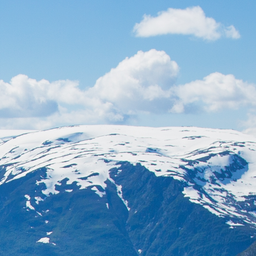
\includegraphics[width=\linewidth]{inc/analysis/noises/original.png}
      \caption{Исходное изображение}
    \end{subfigure} &
    \begin{subfigure}{0.45\textwidth}
      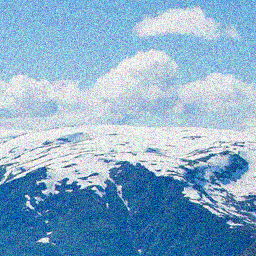
\includegraphics[width=\linewidth]{inc/analysis/noises/gaussian.png}
      \caption{Зашумленное изображение}
    \end{subfigure} \\
  \end{tabular}
  \caption{Шум Гаусса}
  \label{fig:gaussian_noise}
\end{figure}

\textit{\textbf{Солевой и перечный шум}}. Этот тип шума проявляется в виде беспорядочно разбросанных пикселей максимальной интенсивности на изображении, т.е. характеризуется наличием изолированных пикселей с экстремальными значениями интенсивности. Эти пиксели могут значительно исказить внешний вид изображения и нарушить его визуальное восприятие человеком \cite{noisetypes}.

Данный шум может быть описан следующей функцией плотности вероятности:

\noindent
\begin{equation}
    f(x) = p_{\text{salt}} \delta(x - v_{\text{salt}}) + p_{\text{pepper}} \delta(x - v_{\text{pepper}}),
\end{equation}
где
\begin{itemize}
    \item $f(x)$ --- функция плотности вероятности шума;
    \item $x$ --- значение шума;
    \item $p_{\text{salt}}$ и $p_{\text{pepper}}$ --- вероятности пикселей <<соль>> и <<перец>>, соответственно;
    \item $\delta(x)$ --- дельта-функция Дирака, математическая функция, которая равна 0 везде, кроме точки 0, где она бесконечна;
    \item  $v_{\text{salt}}$ и $v_{\text{pepper}}$ --- значения интенсивности <<солевого>> и <<перечного>> пикселей, соответственно.
\end{itemize}

Часто встречается на изображениях, полученных низкокачественными датчиками, например, в камерах наблюдения или в условиях недостаточной освещенности. Он также может быть вызван другими факторами, например, электронными помехами или повреждением данных.

На рисунке \ref{fig:saltpepper_noise} представлен пример солевого и перечного шума.

\begin{figure}[h!]
  \centering
  \begin{tabular}{cc}
    \begin{subfigure}{0.45\textwidth}
      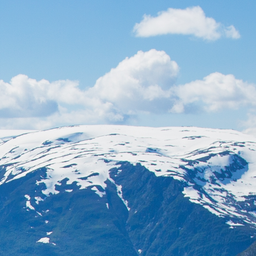
\includegraphics[width=\linewidth]{inc/analysis/noises/original.png}
      \caption{Исходное изображение}
    \end{subfigure} &
    \begin{subfigure}{0.45\textwidth}
      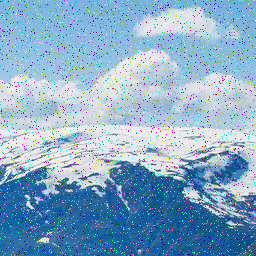
\includegraphics[width=\linewidth]{inc/analysis/noises/saltpepper.png}
      \caption{Зашумленное изображение}
    \end{subfigure} \\
  \end{tabular}
  \caption{Солевой и перечный шум}
  \label{fig:saltpepper_noise}
\end{figure}

\textit{\textbf{Спекл-шум}}. Спекл-шум, также известный как мультипликативный шум или когерентный шум, --- это тип шума, который часто встречается на изображениях, полученных с помощью систем когерентной визуализации. Он характеризуется наличием небольших, беспорядочно распределенных светлых или темных пятен на изображении, часто называемых <<крапинками>> \cite{noisetypes}.

Данный вид шума присутствует на ультразвуковых изображениях, где он вызван интерференцией ультразвуковых волн, отраженных от различных структур в теле.

На рисунке \ref{fig:speckle_noise} представлен пример спекл-шума.

\begin{figure}[h!]
  \centering
  \begin{tabular}{cc}
    \begin{subfigure}{0.45\textwidth}
      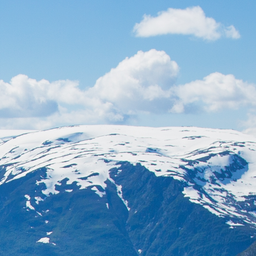
\includegraphics[width=\linewidth]{inc/analysis/noises/original.png}
      \caption{Исходное изображение}
    \end{subfigure} &
    \begin{subfigure}{0.45\textwidth}
      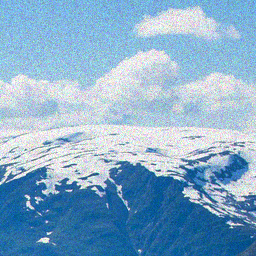
\includegraphics[width=\linewidth]{inc/analysis/noises/speckle.png}
      \caption{Зашумленное изображение}
    \end{subfigure} \\
  \end{tabular}
  \caption{Спекл-шум}
  \label{fig:speckle_noise}
\end{figure}

Задача удаления помех изображений является интересной областью исследований на протяжении десятилетий. За прошедшие годы было предложено множество методов и идей для их устранения. Большинство этих методов предполагают, что шумы в изображениях принадлежат конкретному типу.

Но это предположение не совсем справедливо для реального шума. Реальный шум более сложен и разнообразен (см. рисунок \ref{fig:real_noise}). В связи с этим большинство методов плохо справляются с удалением реального шума с изображений. Поэтому для решения данной проблемы с изображений необходимо использовать более совершенные методы.

\begin{figure}[h!]
  \centering
  \begin{tabular}{cc}
    \begin{subfigure}{0.45\textwidth}
      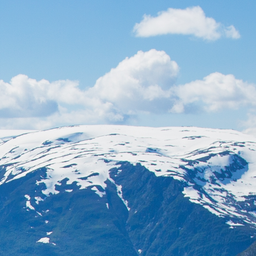
\includegraphics[width=\linewidth]{inc/analysis/noises/original.png}
      \caption{Исходное изображение}
    \end{subfigure} &
    \begin{subfigure}{0.45\textwidth}
      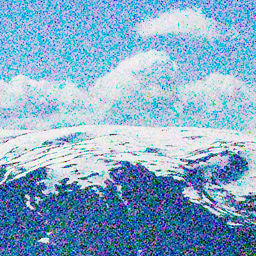
\includegraphics[width=\linewidth]{inc/analysis/noises/real.png}
      \caption{Зашумленное изображение}
    \end{subfigure} \\
  \end{tabular}
  \caption{Реальные шумы}
  \label{fig:real_noise}
\end{figure}

\section{Методы фильтрации шумов на изображениях}

\subsection{Метод среднего арифметического}

Фильтр среднего арифметического --- это простой метод фильтрации, который обычно используется для сглаживания изображений и уменьшения влияния шума. Он работает путем замены значения каждого пикселя изображения средним значением окружающих его пикселей\cite{meanfilter}.

Математически фильтр среднего арифметического можно представить в виде следующей формулы:
\begin{equation}
    I_{\text{filtered}}(x,y) = \frac{1}{N^2} \sum_{i=-\frac{N}{2}}^{\frac{N}{2}} \sum_{j=-\frac{N}{2}}^{\frac{N}{2}} \cdot I(x+i,y+j),
\end{equation}
где
\begin{itemize}
    \item $I_{\text{filtered}}(x,y)$ --- изображение, после применения фильтрации;
    \item $I(x,y)$ --- исходное изображение;
    \item $N$ --- размер окна фильтра, обычно является нечетным числом.
\end{itemize}

Фильтр среднего арифметического --- примитивный и неэффективный метод сглаживания изображений и уменьшения шума, т.к. он также может размыть важные детали изображения и привести к искажению цветов. 

\subsection{Метод фильтрации по Гауссу}
Фильтр Гаусса --- это линейный фильтр, который работает путем свертки изображения с ядром, которое представляет собой небольшую матрицу весов. Веса в ядре определяются функцией Гаусса \cite{gaussianfilter}.

Фильтр Гаусса описывается следующим уравнением:
\begin{equation}
    G(x,y) = \frac{1}{2\pi\sigma^2}e^{-\frac{x^2+y^2}{2\sigma^2}},
\end{equation}
где 
\begin{itemize}
    \item $G(x,y)$ --- значение гауссовой функции в позиции $(x,y)$;
    \item $\sigma$ --- стандартное отклонение.
\end{itemize}

Чтобы применить гауссовский фильтр к изображению, выполняется свертка изображения с ядром в каждом из пикселей:

\begin{equation}
I_{i,j}' = \sum_{m=-\infty}^{\infty} \sum_{n=-\infty}^{\infty} I_{i+m,j+n} G_{m,n},
\end{equation}
где 
\begin{itemize}
    \item $I_{i,j}'$ --- значение пикселя в позиции $(i,j)$ после применения гауссова фильтра;
    \item $I_{i+m,j+n}$ --- значение пикселя в позиции $(i+m,j+n)$ в исходном изображении;
    \item $G_{m,n}$ --- значение ядра в позиции $(m,n)$.
\end{itemize}

Гауссовский фильтр обладает рядом свойств, которые делают его полезным для обработки изображений. Одно из этих свойств заключается в том, что он является низкочастотным фильтром, что означает, что его можно использовать для удаления высокочастотных компонентов из изображения, сохраняя при этом низкочастотные компоненты. Еще одним свойством фильтра Гаусса является его разделимость, т.е. он может быть реализован более эффективно путем применения фильтра отдельно в горизонтальном и вертикальном направлениях.

Одно из ограничений гауссовского фильтра заключается в том, что он плохо подходит для сохранения резких краев изображения.

\subsection{Метод медианной фильтрации}

Метод медианной фильтрации работает путем замены значения каждого пикселя изображения медианным значением окружающих его пикселей \cite{medianfilter}. 

Медианное значение --- это среднее значение в наборе значений, такое, что половина значений меньше, а половина значений больше. Использование данной математической операции позволяет исключить из набора пикселей резкие отклонения по интенсивности, что дает существенный выигрыш при устранении помех типа <<соль и перец>>.

Математически медианный фильтр можно представить в виде следующей формулы:

\begin{equation}
    I_{\text{filtered}}(x,y) = m   \begin{pmatrix}
I(x-1,y-1) && I(x,y-1) && I(x+1,y-1) \\
I(x-1,y) && I(x,y) && I(x+1,y) \\
I(x-1,y+1) && I(x,y+1) && I(x+1,y+1)
\end{pmatrix},
\end{equation}
где
\begin{itemize}
    \item $I_{\text{filtered}}(x,y)$ --- изображение, после применения фильтрации;
    \item $I(x,y)$ --- исходное изображение.
\end{itemize}

Эта формула представляет медианный фильтр 3x3, что является обычным размером ядра медианного фильтра. Медианный фильтр может быть расширен до больших размеров ядра путем добавления большего количества окружающих пикселей к набору значений. Следует отметить, что фильтрационное окно может быть произвольной геометрической формы.

\subsection{Метод билатеральной фильтрации}

Билатеральный метод используется для сглаживания изображения с сохранением краев и является модификацией фильтра Гаусса. Устранение помех выполняется путем замены значения каждого пикселя средневзвешенным значением значений близлежащих пикселей, где вес пикселя определяется комбинацией его интенсивности и пространственного расстояния от центрального пикселя \cite{bilateralfilter}.


Данный метод можно описать следующим образом:
\begin{equation}
	I_\text{filtered}(x) = \frac{1}{W_p} \sum_{x_i \in \Omega} I(x_i)f_r(\|I(x_i) - I(x)\|)g_s(\|x_i - x\|),
\end{equation}

\noindent
\begin{equation}
	W_p = \sum_{x_i \in \Omega}{f_r(\|I(x_i) - I(x)\|)g_s(\|x_i - x\|)},
\end{equation}
где
\begin{itemize}
	\item $I_\text{filtered}$ --- изображение, после применения фильтрации;
	\item $I$ --- исходное изображение;
	\item $x$ --- координаты текущего пикселя для фильтрации;
	\item $\Omega$ --- окно с центром в $x$, тогда $x_i \in \Omega$ соседний пиксель;
	\item $f_r$ --- интенсивности пикселей;
	\item $g_s$ --- функция Гаусса.
\end{itemize}

Пиксель просто заменяется взвешенным средним его соседей.
\noindent
\begin{equation}
	w(i, j, k, l) = \exp\left(-\frac{(i - k)^2 + (j - l)^2}{2 \sigma_d^2} - \frac{\|I(i, j) - I(k, l)\|^2}{2 \sigma_r^2}\right),
\end{equation}
где $\sigma_d$ и $\sigma_r$ --- сглаживающие параметры, и $I(i, j)$ и $I(k, l)$ --- интенсивности пикселей $(i, j)$ и $ (k, l)$ соответственно.

После вычисления весов, необходимо нормализовать их:
\begin{equation}
	I_\text{filtered}(i, j) = \frac{\sum_{k, l} I(k, l) w(i, j, k, l)}{\sum_{k, l} w(i, j, k, l)},
\end{equation}
где $I_\text{filtered}$ интенсивность пикселя $(i, j)$ без шума.

За счет учета как пространственного расстояния, так и сходства интенсивности между пикселями билатеральный фильтр эффективно сохраняет края, структурные составляющие и мелкие детали изображения.  

\subsection{Нейронные сети}

В области обработки изображений нейронные сети получили широкое распространение. Они представляют собой мощный инструмент, способный обучаться на основе больших наборов данных и извлекать сложные комплексные характеристики объектов. Это открыло новые возможности в таких задачах, как классификация изображений, обнаружение объектов, сегментация, стилизация и фильтрация \cite{generalimageprocessing}.

В общем виде шумы некоторого изображения могут быть описаны следующим образом:
\begin{equation}
    Y = X + N,
\end{equation}
где $Y$ --- изображение с помехами, $X$ --- истинное изображение, $N$ --- шум. Тогда в случае известной величины $N$ легко восстановить исходное изображение по изображению с помехами:
\begin{equation}
    X = Y - N.
\end{equation}

Нейронные сети предназначены для оценки и извлечения величины шума $N$ на основе изображения $Y$. Они используют несколько слоев нейронов, специально разработанных для обработки изображений. Количество и типы слоев могут варьироваться в зависимости от конкретной реализации нейронной сети.

Преимущества использования нейронных сетей в обработке изображений связаны с их способностью извлекать множество признаков из входных изображений. Это позволяет достичь существенно лучших результатов по сравнению с ранее рассмотренными алгоритмами. Нейронные сети могут эффективно устранять помехи любого вида, сохраняя при этом детали и грани объектов на изображении. Важно отметить, что в отличие от традиционных методов, нейронным сетям не требуется подбор параметров фильтров, так как они обучаются автоматически на основе данных.

Однако качество восстановления изображения зависит от набора данных, на основе которого производилось обучение модели нейронной сети. Хорошо разнообразный и представительный набор данных позволяет модели лучше обобщать и обрабатывать различные типы шума. Поэтому выбор и разработка подходящего набора данных играют важную роль в успешном применении нейронных сетей для восстановления изображений.

В итоге, методы, основанные на нейронных сетях, представляют собой мощный универсальный инструмент для обработки изображений, обеспечивая высокое качество восстановления и фильтрации помех. Постоянные исследования и разработки в этой области направлены на улучшение моделей нейронных сетей, расширение спектра задач и повышение их эффективности в реальных сценариях обработки изображений.

\subsection{Сравнение рассмотренных методов}

На основе приведенной ранее информации составлены сравнительные таблицы \ref{tabular:methods_tasks}--\ref{tabular:methods_features} по задачам и характеристикам рассмотренных методов. Условные обозначения:
\begin{itemize}
    \item MEAN --- метод среднего арифметического;
    \item GAUSSIAN --- метод фильтрации Гаусса;
    \item MEDIAN --- метод медианной фильтрации;
    \item BILATERAL --- метод билатеральной фильтрации.
\end{itemize}

\begin{table}[h!]
	\centering
    \captionsetup{justification=raggedleft,singlelinecheck=false}
	\caption{\label{tabular:methods_tasks} Сравнительная таблица рассмотренных методов по задачам}
\resizebox{\textwidth}{!}{\begin{tabular}{|c|c|c|c|c|c|}
\hline
Задача & MEAN & GAUSSIAN & MEDIAN & BILATERAL & \begin{tabular}[c]{@{}c@{}}Нейронные \\ сети\end{tabular} \\ \hline
\begin{tabular}[c]{@{}c@{}}Устранение шумов \\ Гаусса\end{tabular} & Среднее & Среднее & Среднее & Среднее & Высокое \\ \hline
\begin{tabular}[c]{@{}c@{}}Устранение шумов\\  Соль и Перец\end{tabular} & \begin{tabular}[c]{@{}c@{}}Очень\\  низкое\end{tabular} & Низкое & Высокое & Среднее & Высокое \\ \hline
\begin{tabular}[c]{@{}c@{}}Устранение \\ Спекл-шумов\end{tabular} & Среднее & Среднее & Среднее & Среднее & Высокое \\ \hline
\begin{tabular}[c]{@{}c@{}}Устранение \\ реальных шумов\end{tabular} & \begin{tabular}[c]{@{}c@{}}Очень \\ низкое\end{tabular} & \begin{tabular}[c]{@{}c@{}}Очень \\ низкое\end{tabular} & \begin{tabular}[c]{@{}c@{}}Очень \\ низкое\end{tabular} & Низкое & Высокое \\ \hline
\end{tabular}}
\end{table}

\begin{table}[h!]
	\centering
    \captionsetup{justification=raggedleft,singlelinecheck=false}
	\caption{\label{tabular:methods_features} Сравнительная таблица рассмотренных методов по характеристикам}
\resizebox{\textwidth}{!}{\begin{tabular}{|c|c|c|c|c|c|}
\hline
Характеристика & MEAN & GAUSSIAN & MEDIAN & BILATERAL & \begin{tabular}[c]{@{}c@{}}Нейронные \\ сети\end{tabular} \\ \hline
\begin{tabular}[c]{@{}c@{}}Качество \\ сохранения деталей\end{tabular} & Низкое & Низкое & Низкое & Среднее & Высокое \\ \hline
\begin{tabular}[c]{@{}c@{}}Качество \\ сохранения граней\end{tabular} & Низкое & Низкое & Среднее & Высокое & Высокое \\ \hline
\begin{tabular}[c]{@{}c@{}}Универсальность \\ параметров\end{tabular} & Средняя & Средняя & Средняя & Средняя & Высокая \\ \hline
\end{tabular}}
\end{table}

Таким образом, для реализации собственного метода фильтрации малоразмерных помех будут использоваться нейронные сети ввиду преимущества по большинству параметров методов, основанных на них.

\section{Нейронные сети}

Биологические нейроны являются основными строительными блоками нервной системы живых существ, включая человека. Они обрабатывают информацию и передают ее другим нейронам через электрохимические сигналы, называемые импульсами. Нейронные сети в компьютерной науке моделируют работу биологических нейронов, используя математические алгоритмы и структуры данных.

Нейронные сети --- это компьютерные модели, разработанные для имитации работы человеческого мозга и его нейронной системы. Они используются для решения различных задач машинного обучения, включая классификацию, распознавание образов, прогнозирование, обработку естественного языка и многое другое.

Нейронная сеть состоит из множества искусственных нейронов, которые соединены между собой. Они образуют слои, пропуская данные от входного слоя к выходному слою. Основные составляющие элементы нейронной сети включают:

\begin{itemize}
    \item \textit{Нейроны}. Искусственные нейроны или узлы являются основными вычислительными единицами нейронной сети. Они получают входные сигналы, обрабатывают их и генерируют выходной сигнал на основе активационной функции. Каждый нейрон имеет свои веса и смещение, которые определяют его поведение.
    \item \textit{Связи}. Связи представляют собой каналы передачи данных между нейронами. У каждой связи есть свой вес, который определяет ее силу или важность при передаче данных.
    \item \textit{Слои}. Нейронные сети обычно имеют несколько слоев, включая входной слой, скрытые слои и выходной слой. Входной слой получает входные данные, скрытые слои обрабатывают данные и выходной слой генерирует окончательный результат или прогноз.
    \item \textit{Активационная функция}. Активационная функция определяет выходной сигнал нейрона на основе его входных данных. Она может быть линейной или нелинейной и обеспечивает нейронной сети способность моделировать сложные нелинейные отношения.
\end{itemize}

Структурная схема нейронной сети описывается следующими слоями: входной слой, скрытые слои, выходной слой (см. рисунок \ref{fig:simple_net}).

\begin{figure}[h!btp]
	\centering
	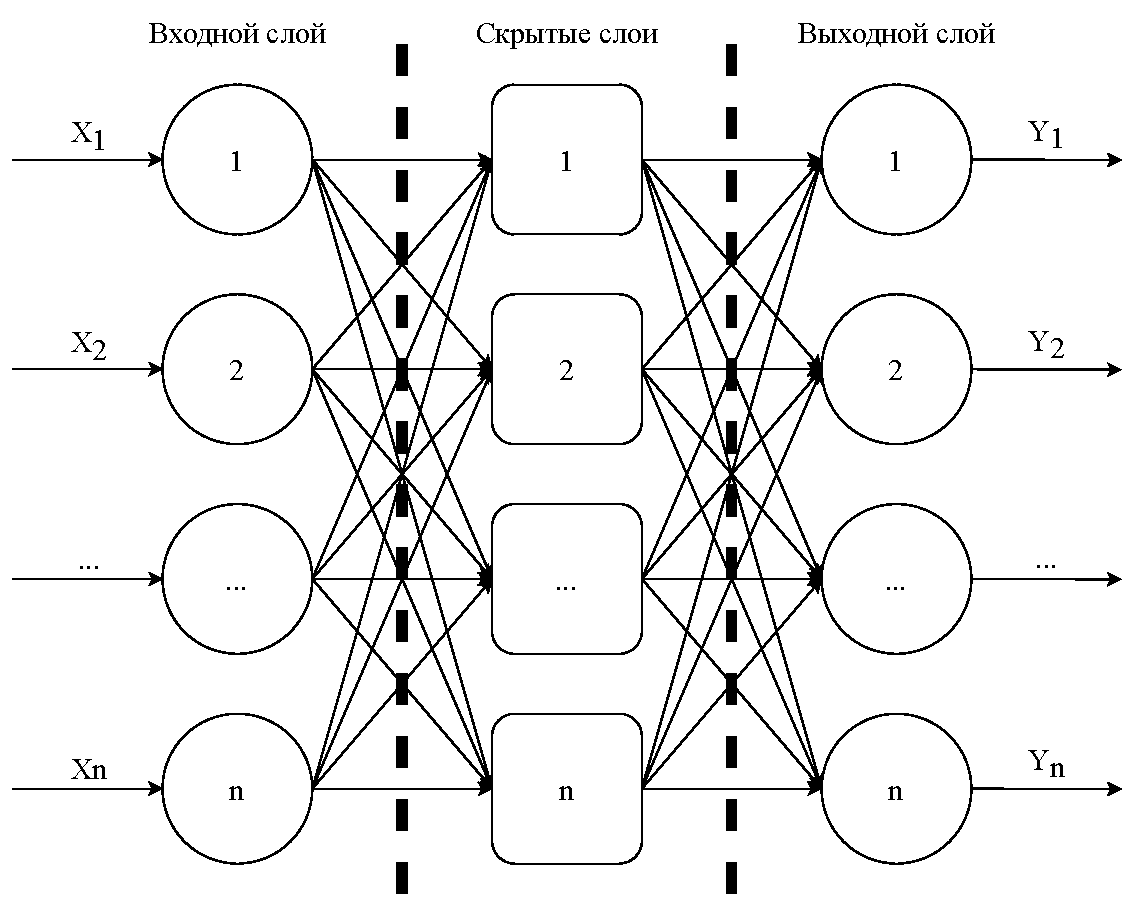
\includegraphics[scale = 0.7]{inc/analysis/simple_net.pdf}
	\caption{Общая схема нейронной сети}
	\label{fig:simple_net}	
\end{figure}

Входной слой является первым слоем нейронной сети, который принимает входные данные. Количество нейронов в этом слое соответствует количеству признаков или размерности входных данных.

Скрытые слои находятся между входным и выходным слоями. Количество скрытых слоев и количество нейронов в каждом слое зависят от архитектуры нейронной сети. Скрытые слои выполняют промежуточную обработку данных, извлекая признаки и выявляя сложные зависимости в данных.

Выходной слой --- это последний слой нейронной сети, который генерирует выходные данные или предсказания. Количество нейронов в выходном слое зависит от задачи, которую решает нейронная сеть. Например, для задачи бинарной классификации может быть один нейрон, а для задачи многоклассовой классификации может быть несколько нейронов.

Кроме основных элементов, в некоторых архитектурах нейронных сетей могут присутствовать и дополнительные компоненты, такие как рекуррентные связи для обработки последовательных данных во времени или сверточные слои для анализа пространственных шаблонов в данных.

Структура нейронной сети может быть глубокой (с большим количеством скрытых слоев) или неглубокой (с одним или несколькими скрытыми слоями). В зависимости от задачи и доступных данных, разные архитектуры нейронных сетей могут быть эффективными для различных приложений.

\subsection{Принцип работы нейронной сети}

В основе работы нейронной сети лежит модель линейной регрессии, применяемая к каждому узлу сети. Каждый узел представляет собой модель линейной регрессии, которая объединяет входные данные, весовые коэффициенты, смещение (или пороговое значение) и выходные данные \cite{neuralnetworkswork}.

Уравнение для модели линейной регрессии в узле выглядит следующим образом:

\begin{equation}
\hat{y} = \sum_{i=1}^{m}w_ix_i + bias,
\end{equation}

где
\begin{itemize}
    \item $\hat{y}$ --- прогнозируемое значение модели;
    \item $m$ --- количество факторов (входных данных);
    \item $w$ --- весовой коэффициент фактора;
    \item $x$ --- входные данные;
    \item $bias$ --- смещение (ошибка).
\end{itemize}

Для определения выходного значения узла применяется функция активации.

Процесс работы нейронной сети включает следующие шаги:
\begin{enumerate}
    \item Определение слоя входных данных.
    \item Назначение весовых коэффициентов, которые определяют важность каждого фактора.
    \item Умножение входных данных на соответствующие весовые коэффициенты и их суммирование.
    \item Применение функции активации к полученной сумме для вычисления результата и определения активации узла.
    \item Передача выходных данных активированного узла на следующий слой нейронной сети.
    \item Повторение шагов 2-5 для каждого узла и каждого слоя до достижения выходного слоя.
\end{enumerate}

Таким образом, нейронная сеть прямого распространения последовательно передает данные через слои, где каждый узел работает на основе модели линейной регрессии и функции активации. Этот процесс и позволяет сети извлекать и обрабатывать информацию для решения задач классификации, регрессии и других.

\subsection{Функции активации}

Функции активации играют важную роль в передаче сигнала через нейроны нейронных сетей \cite{activations}. Они определяют активацию нейронов и влияют на выходные значения нейронов, которые передаются следующим слоям сети.

\textit{Сигмоидная функция активации} представляется с помощью следующего уравнения:
\begin{equation}
   f(x) = \frac{1}{{1 + e^{-x}}}.
\end{equation}
Данная функция преобразует входные значения в вероятности или величины, близкие к 0 или 1. Широко использовалась в прошлом для бинарной классификации, но имеет проблему исчезающего градиента.

\textit{Функция активации гиперболического тангенса} имеет вид:
\begin{equation}
   f(x) = \frac{{e^x - e^{-x}}}{{e^x + e^{-x}}}.
\end{equation}
Роль аналогична сигмоидной функции, но со сдвигом и более крутым градиентом. Широко используется в рекуррентных нейронных сетях.

\textit{Функция ReLU}:
\begin{equation}
f(x) = \max(0, x).
\end{equation}
Очень популярная функция активации в сверточных нейронных сетях. Активирует нейроны при положительных значениях входа и неактивна при отрицательных значениях, что способствует разреженности активаций и более эффективному обучению.

\textit{Линейная функция активации} не вводит нелинейность и используется в задачах регрессии, где требуется предсказание непрерывных значений:
\begin{equation}
   f(x) = x.
\end{equation}

Это лишь несколько примеров функций активации, и существуют и другие. Выбор функции активации зависит от архитектуры сети, типа задачи и требуемого поведения нейронов. Правильный выбор функции активации может помочь нейронной сети достичь лучших результатов и ускорить ее обучение.

\subsection{Обучение нейронной сети}

Обучение нейронной сети является процессом настройки параметров сети путем моделирования окружающей среды, в которую эта сеть встраивается. Способ настройки параметров определяет тип обучения, который может быть с учителем или без учителя. На рисунке \ref{fig:learning} представлена общая схема обучения нейронной сети. 

\begin{figure}[h!btp]
	\centering
	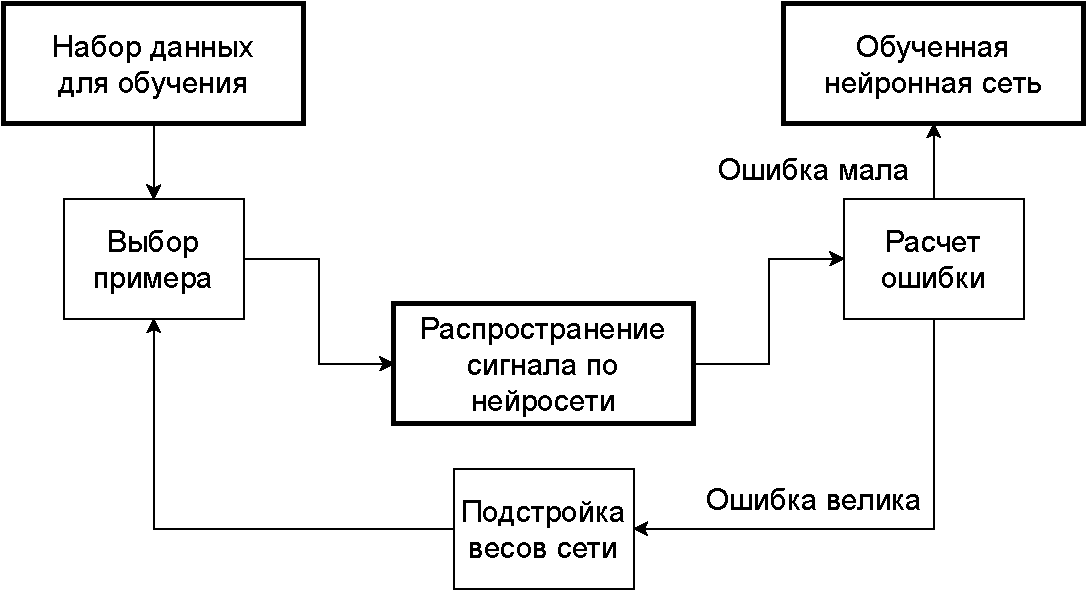
\includegraphics[scale = 0.8]{inc/analysis/learning.pdf}
	\caption{Общая схема обучения нейронной сети}
	\label{fig:learning}	
\end{figure}

В процессе \textbf{обучения с учителем} сети предъявляется набор обучающих примеров. Каждый пример подается на входы сети, затем проходит обработку внутри структуры нейронной сети, вычисляется выходной сигнал сети. Этот выходной сигнал сравнивается с соответствующим значением целевого вектора, который представляет требуемый выход сети. Таким образом, обучение с учителем заключается в настройке параметров нейронной сети на основе сравнения выходов сети с ожидаемыми целевыми значениями. Далее, на основе определенного правила, вычисляется ошибка, и весовые коэффициенты связей внутри сети изменяются в соответствии с выбранным алгоритмом. Процесс предъявления обучающих векторов, вычисления ошибок и подстройки весов продолжается последовательно до достижения приемлемо низкого уровня ошибки по всему обучающему набору.

Таким образом, обучение с учителем заключается в постепенной подстройке весовых коэффициентов нейронной сети на основе последовательного предъявления обучающих векторов, вычисления ошибок и корректировки весов для достижения низкого уровня ошибки по всему обучающему набору.

При \textbf{обучении без учителя} обучающее множество состоит только из входных векторов, без соответствующих целевых значений. Обучающий алгоритм подстраивает веса сети таким образом, чтобы выходные векторы были согласованы, то есть предъявление достаточно близких входных векторов давало одинаковые выходы. Процесс обучения, следовательно, выявляет статистические свойства обучающего множества и группирует схожие векторы в классы.

На сегодняшний день в свободном доступе существует большое количество изображений, полученных в разных условиях и уровнем качества, на основе которых может быть проведено обучение с учителем без необходимости выявления статистических свойств в обучающей выборке.

\subsection{Функции потерь}

Функции потерь (или функции ошибки) используются при обучении для оценки качества работы нейронной сети путем сравнения ее предсказанных значений с фактическими значениями. Вот некоторые распространенные функции потерь и их использование \cite{losses}:

1. Среднеквадратичная ошибка:
\begin{equation}
   \text{MSE} = \frac{1}{N}\sum_{i=1}^{N}(y_i - \hat{y}_i)^2.
\end{equation}
Часто используется в задачах регрессии, обработки изображений, аудио, видео, где требуется предсказание непрерывных значений. Данная функция потерь стремится минимизировать среднеквадратичную разницу между предсказанными и фактическими значениями.

2. Категориальная перекрестная энтропия:
\begin{equation}
   \text{CE} = -\sum_{i=1}^{N}y_i \log(\hat{y}_i).
\end{equation}
Широко используется в задачах многоклассовой классификации, где требуется предсказание вероятностей для каждого класса. Данная функция потерь стремится минимизировать разницу между предсказанными и фактическими вероятностями классов.

3. Бинарная перекрестная энтропия:
\begin{equation}
   \text{CE} = -y \log(\hat{y}) - (1-y) \log(1-\hat{y}).
\end{equation}
Часто используется в задачах бинарной классификации, где требуется предсказание вероятности для двух классов. Данная функция потерь стремится минимизировать разницу между предсказанными и фактическими вероятностями классов.

4. Средняя абсолютная ошибка:
\begin{equation}
   \text{MAE} = \frac{1}{N}\sum_{i=1}^{N}|y_i - \hat{y}_i|.
\end{equation}
Альтернатива среднеквадратичной ошибки в задачах регрессии.

Каждая функция потерь имеет свои особенности и подходит для конкретных типов задач и данных. Выбор правильной функции потерь влияет на эффективность обучения и качество предсказаний нейронной сети.

\subsection{Метод обратного распространения ошибки}

Метод обратного распространения ошибки является основным алгоритмом для обучения глубоких нейронных сетей \cite{backpropagation}. Он позволяет вычислить градиент функции потерь по всем весам сети и использовать его для обновления весов на каждом слое.

Пусть у нас есть нейронная сеть с \(L\) слоями, \(w_{ij}^l\) обозначает вес между нейронами \(i\)-го и \(j\)-го слоя на \(l\)-ом слое, \(a_i^l\) --- активация \(i\)-го нейрона на \(l\)-ом слое, а \(b_i^l\) --- смещение \(i\)-го нейрона на \(l\)-ом слое.

Обратное распространение ошибки состоит из двух этапов: прямого и обратного прохода.

\textit{Прямой проход} состоит в том, что для каждого нейрона на каждом слое сети вычисляется активация с помощью активационной функции. Активации передаются последовательно от входного слоя к выходному слою, что позволяет получить предсказания сети.

Во время \textit{обратного прохода} вычисляется градиент функции потерь по активациям последнего слоя сети. Обозначим этот градиент как \(\delta^{L}\). В зависимости от задачи и используемой функции потерь, формула для \(\delta^{L}\) будет разной. По цепочке вычисляются градиенты по активациям на предыдущих слоях сети. Для каждого слоя \(l\), градиент по активациям на \(l\)-ом слое (\(\delta^l\)) вычисляется по формуле: 
\begin{equation}
    \delta^l = ((w^{l+1})^T \delta^{l+1}) \odot \sigma'(z^l),
\end{equation}
где \(\odot\) --- поэлементное умножение, \(\sigma'(z^l)\) --- производная активационной функции по взвешенной сумме входов нейронов на \(l\)-ом слое. Градиенты по весам и смещениям вычисляются с использованием градиента по активациям. Так градиент по весу между нейронами \(i\) и \(j\) на \(l\)-ом слое будет равен: 
\begin{equation}
    \frac{\partial J}{\partial w_{ij}^l} = a_j^{l-1} \delta_i^l.
\end{equation}

\subsection{Виды нейронных сетей}

Существует достаточно большое количество видов нейронных сетей, например, нейросети прямого распространения, рекуррентные нейронные сети, сверточные нейронные сети, самоорганизующиеся карты, капсульные нейронные сети. Каждый из этих типов имеет свои особенности и применяется для решения определенных задач, таких как классификация, обработка образов и кластеризация данных \cite{neurotypes}.

\textit{Нейросети прямого распространения} \cite{ffn} (см. рисунок \ref{fig:simple_net}):
\begin{itemize}
    \item прямое распространение является наиболее базовым типом нейронных сетей. Он состоит из одного или нескольких скрытых слоев нейронов, а также входного и выходного слоев;
    \item сигнал движется от входного слоя к выходному слою без обратной связи;
    \item входные данные передаются через слои с помощью весов, а на каждом слое применяется функция активации;
    \item широко используется для задач классификации и регрессии.
\end{itemize}

\textit{Рекуррентные нейронные сети} \cite{recurrent}:
\begin{itemize}
    \item предназначены для работы с последовательными данными, где входные данные имеют зависимость от предыдущих шагов;
    \item наличие циклических и обратных связей, позволяет сохранять информацию о предыдущих состояниях;
    \item применяются в задачах обработки естественного языка, машинного перевода, распознавания речи и временных рядов.
\end{itemize}

\textit{Сверточные нейронные сети} \cite{cnns} (см. рисунок \ref{fig:cnn}):
\begin{itemize}
    \item оптимизированы для обработки структурированных данных, например, изображений;
    \item они состоят из слоев свертки, пулинга и полносвязных слоев.
    \item сверточные слои используют фильтры для обнаружения локальных особенностей в изображении;
    \item пулинговые слои уменьшают размерность предыдущего слоя, усредняя или выбирая максимальные значения;
    \item широко применяются в задачах компьютерного зрения, включая классификацию изображений, сегментацию и обнаружение объектов.
\end{itemize}

\textit{Самоорганизующиеся карты} \cite{soms}:
\begin{itemize}
    \item являются нейронными сетями, используемыми для кластеризации и визуализации данных;
    \item они позволяют найти структуру в неупорядоченных данных и проектировать их на двухмерное пространство;
    \item состоит из слоя нейронов, которые организованы на сетке. Нейроны соседствуют друг с другом и образуют топологию, отражающую внутреннюю структуру данных.
\end{itemize}

\textit{Капсульные нейронные сети} \cite{capsules}:
\begin{itemize}
    \item являются относительно новым подходом в области глубокого обучения и предложены для улучшения моделирования пространственных иерархических отношений в данных;
    \item состоят из капсул --- группы нейронов, которые представляют собой кластеры активаций, которые кодируют различные свойства объектов, такие как положение, размер, угол, т.е. занимаются извлечением и представлением многомерных характеристик объектов, в отличие от обычных нейронов, которые представляют собой скалярные значения;
    \item вместо передачи активации от одного слоя к другому, как в обычных нейросетях, капсульные нейросети используют динамическую маршрутизацию для передачи информации между капсулами;
    \item в капсульных нейросетях, капсулы активируются с помощью скалярного произведения между входными данными и предсказанными параметрами капсулы. Это позволяет капсулам кодировать информацию о присутствии или отсутствии объектов, а также об их характеристиках;
    
\end{itemize}

В таблице \ref{tabular:nets} представлено сравнение рассмотренных видов нейронных сетей.

\begin{table}[h!]
	\centering
    \captionsetup{justification=raggedleft,singlelinecheck=false}
	\caption{\label{tabular:nets} Сравнительная таблица видов нейронных сетей}
 
\resizebox{\textwidth}{!}{\begin{tabular}{|c|c|c|c|c|c|}
\hline
Критерий & \begin{tabular}[c]{@{}c@{}}Нейросети\\ прямого\\ распространения\end{tabular} & \begin{tabular}[c]{@{}c@{}}Рекуррентные\\ нейросети\end{tabular} & \begin{tabular}[c]{@{}c@{}}Сверточные\\ нейросети\end{tabular} & \begin{tabular}[c]{@{}c@{}}Самоорганизующиеся\\ карты\end{tabular} & \begin{tabular}[c]{@{}c@{}}Капсульные \\ нейросети\end{tabular} \\ \hline
Архитектура & \begin{tabular}[c]{@{}c@{}}Последовательные\\ слои\end{tabular} & \begin{tabular}[c]{@{}c@{}}Рекуррентные\\ связи\end{tabular} & \begin{tabular}[c]{@{}c@{}}Сверточные\\ слои\end{tabular} & \begin{tabular}[c]{@{}c@{}}Самоорганизация \\ на основе кластеров\end{tabular} & \begin{tabular}[c]{@{}c@{}} Слои \\ с капсулами \end{tabular} \\ \hline
\begin{tabular}[c]{@{}c@{}}Определение\\ пространственных\\ структур\end{tabular} & Низкое & Низкое & Высокое & Низкое & Высокое \\ \hline
\begin{tabular}[c]{@{}c@{}}Вычислительная\\ эффективность\end{tabular} & Высокая & Средняя & Высокая & Средняя & Средняя \\ \hline
\begin{tabular}[c]{@{}c@{}}Затраты по\\ памяти\end{tabular} & Низкие & Высокие & Средние & Средние & Средние \\ \hline
\begin{tabular}[c]{@{}c@{}}Области \\ применения\end{tabular} & \begin{tabular}[c]{@{}c@{}}Классификация \\ и регрессия\end{tabular} & \begin{tabular}[c]{@{}c@{}}Обработка\\ текста\end{tabular} & \begin{tabular}[c]{@{}c@{}}Обработка\\ изображений\\ и видео\end{tabular} & \begin{tabular}[c]{@{}c@{}}Кластеризация и\\ визуализация\\ данных\end{tabular} & \begin{tabular}[c]{@{}c@{}}Распознавание \\ объектов\end{tabular} \\ \hline
\end{tabular}}
\end{table}

Таким образом, для решения поставленной задачи наиболее соответствует архитектура сверточных нейронных сетей, более того, она оптимизирована для обработки структурированных данных, таких как изображения.

\newpage

\subsection{Критерии выбора данных для обучения нейронной сети}

При выборе данных для обучения нейронной сети, предназначенной для фильтрации шумов на изображениях, следует учитывать несколько критериев, чтобы обеспечить эффективное и точное обучение:

\begin{enumerate}
    \item Представительность данных: данные должны быть представительными для реальных сценариев или задач, которые предполагается решать с помощью нейронной сети.
    \item Разнообразие данных: важно обеспечить разнообразие данных, чтобы нейронная сеть могла обобщать и распознавать паттерны в различных ситуациях. Разнообразие может включать различные условия освещения, углы съемки, фоновые объекты и т. д. Это помогает предотвратить переобучение и обеспечить обобщающую способность сети.
    \item Наличие чистых и зашумленных изображений: помимо шумовых изображений, необходимо иметь доступ к исходным чистым версиям этих изображений. Это позволит сравнить выходные результаты нейронной сети с оригинальными данными и оценить ее эффективность в устранении шумов.
    \item Размер выборки данных: объем данных также играет важную роль. Больший объем данных позволяет нейронной сети лучше обобщать и находить общие закономерности в шумовых изображениях. Оптимальный размер выборки будет зависеть от сложности задачи и доступных ресурсов.
    \item Доступность и этичность данных: важно убедиться, что выбранные данные доступны для использования и что их использование соблюдает правовые и этические нормы. Необходимо учитывать приватность и конфиденциальность данных и убедиться, что выбранный набор данных соответствует требованиям и политикам в области защиты данных.
\end{enumerate}

Учитывая вышеперечисленные критерии, следует стремиться использовать набор данных, тщательный выбор данных способствует созданию надежной и эффективной нейронной сети для фильтрации шумов на изображениях, что в результате приводит к улучшению качества и повышению эффективности работы системы.

\section{Архитектуры сверточных нейронных сетей}

\subsection{Классический подход}

Классическая архитектура сверточной нейронной сети обычно состоит из конволюционных слоев, слоев объединения (пуллинга) и полностью связанных слоев.

\begin{figure}[h!btp]
	\centering
	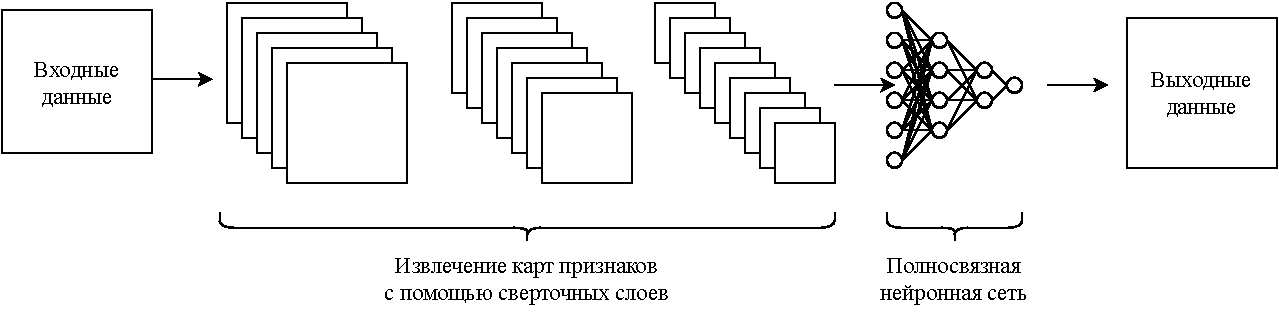
\includegraphics[scale = 0.75]{inc/analysis/cnn.pdf}
	\caption{Схема сверточной нейронной сети}
	\label{fig:cnn}	
\end{figure}

\textit{Входной слой} получает необработанные данные изображения в качестве входных данных. Размер входного слоя определяется размерами входных изображений.

\textit{Конволюционные слои} состоят из нескольких фильтров или ядер, которые скользят по входному изображению. Каждый фильтр выполняет операцию свертки, вычисляя точечные произведения между своими весами и локальными входными данными. На выходе сверточного слоя получается набор карт признаков, которые отражают локальные особенности входного изображения. В качестве функции активации обычно применяются нелинейные методы, например, ReLU.

\textit{Слои объединения} уменьшают пространственные размеры карт признаков, сохраняя при этом наиболее важную информацию:
\begin{enumerate}
    \item MaxPooling выбирает максимальное значение для каждого окна объединения.
    \begin{equation}
        \text{MaxPooling}(x) = \max(x_{i,j}).
    \end{equation}
    \item AvgPooling выбирает среднее значение для каждого окна объединения.
    \begin{equation}
        \text{AvgPooling}(x) = \frac{1}{N}\sum_{i,j}x_{i,j}.
    \end{equation}
\end{enumerate}

\textit{Полностью связанные слои} соединяют каждый нейрон в одном слое с каждым нейроном в следующем слое. Они обрабатывают карты признаков, полученные от предыдущих слоев. Полностью связанные слои отвечают за изучение глобальных закономерностей и составление окончательных прогнозов.

\textit{Выходной слой} производит окончательные прогнозы или классификации на основе входного изображения. Количество нейронов в выходном слое зависит от конкретной задачи.

\subsection{FCN}

Полностью конволюционные нейронные сети (FCN) --- это тип архитектуры сверточных нейронных сетей, специально разработанный для точных прогнозов, таких как семантическая сегментация, в которой каждому пикселю присваивается метка класса \cite{fcns}. В отличие от традиционных нейронных сетей, которые заканчиваются полносвязными слоями, полностью конволюционные нейронные сети заменяют эти полносвязные слои свертками 1x1 (см. рисунок \ref{fig:fcn_scheme}). Данный вид сверточных нейронных сетей позволяет извлекать подробную информацию из изображений и анализировать их на высоком уровне. 

\begin{figure}[h!btp]
	\centering
	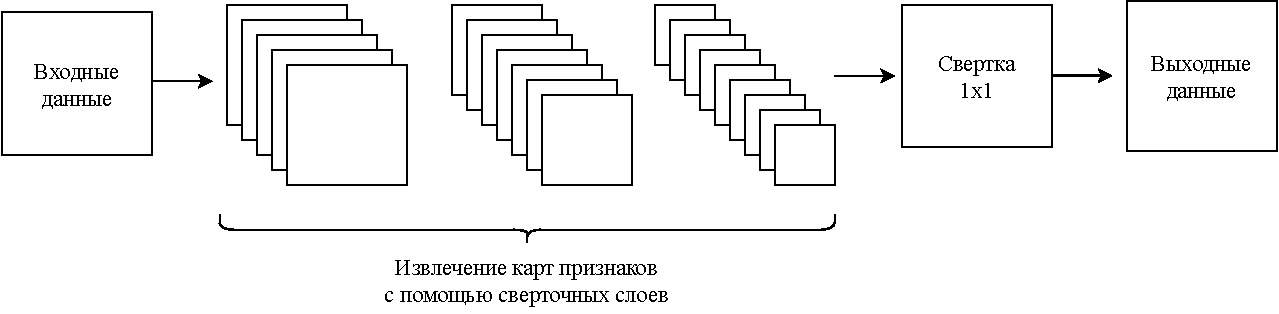
\includegraphics[scale = 0.75]{inc/analysis/fcn_scheme.pdf}
	\caption{Схема полностью сверточной нейронной сети}
	\label{fig:fcn_scheme}	
\end{figure}

Данный тип нейронных сетей состоит только из конволюционных слоев, которые отвечают за извлечение признаков. Эти слои используют ядра свертки для сканирования входного изображения и извлечения соответствующих характеристик. Каждый фильтр выполняет операцию свертки, беря небольшое рецептивное поле и вычисляя точечное произведение с соответствующей областью на входе. Несколько фильтров применяются для захвата различных особенностей в различных пространственных точках изображения.

Уменьшение выборки обычно достигается с помощью слоев объединения, таких как максимальное или среднее объединение, которые уменьшают пространственные размеры карт признаков, сохраняя при этом важные признаки. Уменьшение выборки помогает извлечь высокоуровневую и глобальную контекстную информацию.

С другой стороны, повышение разрешения необходимо для того, чтобы вернуть карты признаков к исходному разрешению. Используются методы повышения разрешения, такие как транспонированные свертки или билинейная интерполяция, для восстановления пространственных деталей, потерянных при пуллинге.

\subsection{UNet}

UNet является развитием FCN и одной из стандартных архитектур сверточных нейронных сетей для задач обработки изображений \cite{unets}. Ее основное применение --- это классификация изображений в целом и разделение их на области по классам (сегментация экземпляров). Архитектура сети состоит из двух основных частей: сжимающего пути, который служит для извлечения контекста, и расширяющегося пути, который обеспечивает точную локализацию. Структура данной нейронной сети приведена на рисунке \ref{fig:unet_classic}.

\begin{figure}[h!btp]
	\centering
	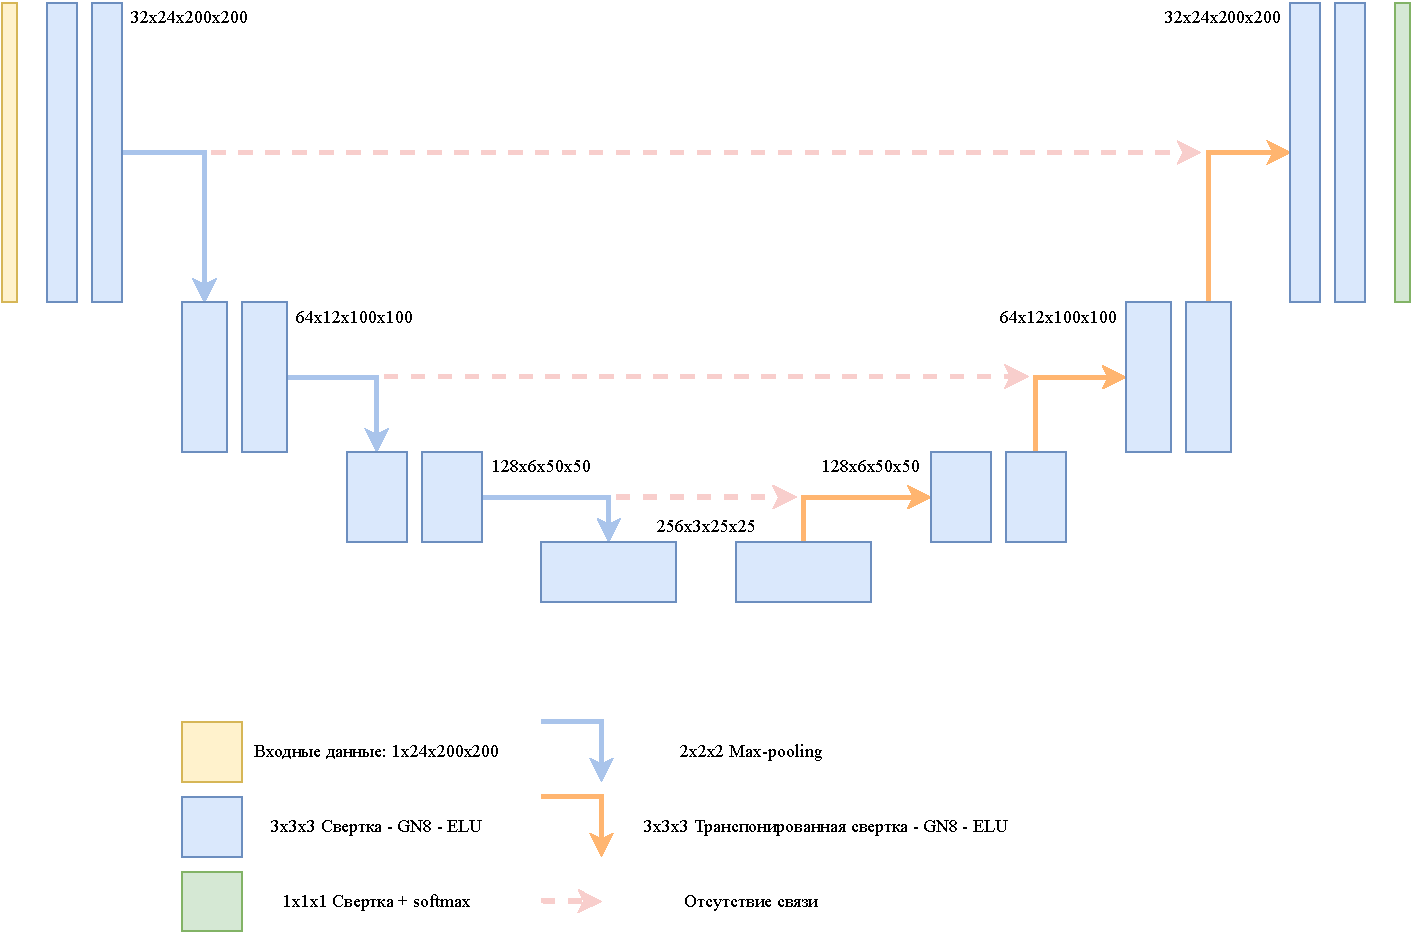
\includegraphics[scale = 0.65]{inc/analysis/unet.pdf}
	\caption{Классическая структура нейронной сети UNet}
	\label{fig:unet_classic}	
\end{figure}

Сжимающий путь включает последовательное применение двух сверток 3x3, за которыми следует функция активации ReLU и операция максимального объединения для уменьшения разрешения. На каждом уровне сжатия, количество признаков удваивается. Каждый шаг в расширяющемся пути включает операцию повышения разрешения карты признаков, за которой следуют свертка 2x2, которая уменьшает количество признаков; объединение с обрезанной картой признаков из сжимающего пути и две свертки 3x3, за которыми следует функция активации ReLU.

На последнем слое применяется свертка 1x1 для сопоставления каждого 64-компонентного вектора признаков с требуемым количеством классов. В общей сложности, сеть UNet содержит 23 сверточных слоя.

UNet показывает высокую производительность и широко используется в различных задачах обработки изображений, например, в мединской сегментации органов на снимках. Ее способность захватывать как глобальный контекст, так и мелкие детали с помощью пропущенных соединений между сжимающим и расширяющимся путями делает ее эффективным инструментом для точного решения задач обработки изображений.

\subsection{Сравнение рассмотренных архитектур}
В таблице \ref{tabular:archs} приведено сравнение рассмотренных архитектур сверточных нейронных сетей. В качестве основы для разрабатываемого метода устранения шумов будет использоваться архитектура UNET, ввиду ее преимущества по всем параметрам.
\begin{table}[h!]
	\centering
    \captionsetup{justification=raggedleft,singlelinecheck=false}
	\caption{\label{tabular:archs} Сравнительная таблица архитектур}
	\begin{tabular}{|c|c|c|c|}
    \hline
    Критерий & \begin{tabular}[c]{@{}c@{}}Классическая\\ архитектура\end{tabular} & FCN & UNET \\ \hline
    \begin{tabular}[c]{@{}c@{}}Вычислительная\\ сложность\end{tabular} & Средняя & Низкая & Средняя \\ \hline
    \begin{tabular}[c]{@{}c@{}}Общее понимание\\ сцены\end{tabular} & + & + & + \\ \hline
    \begin{tabular}[c]{@{}c@{}}Сохранение\\ детализации\end{tabular} & - & - & + \\ \hline
    \begin{tabular}[c]{@{}c@{}}Выявление \\ шумов\\ \end{tabular} & + & + & + \\ \hline
    \begin{tabular}[c]{@{}c@{}}Устранение \\ шумов\\ \end{tabular} & + & - & + \\ \hline
    \end{tabular}
\end{table}

\section{Формализация задачи}

Для формализации задачи используется IDEF0--диаграмма нулевого уровня, которая включает в себя общую цель системы. На рисунке \ref{fig:idef0_0} представлена соответствующая диаграмма.

\begin{figure}[h!btp]
	\centering
	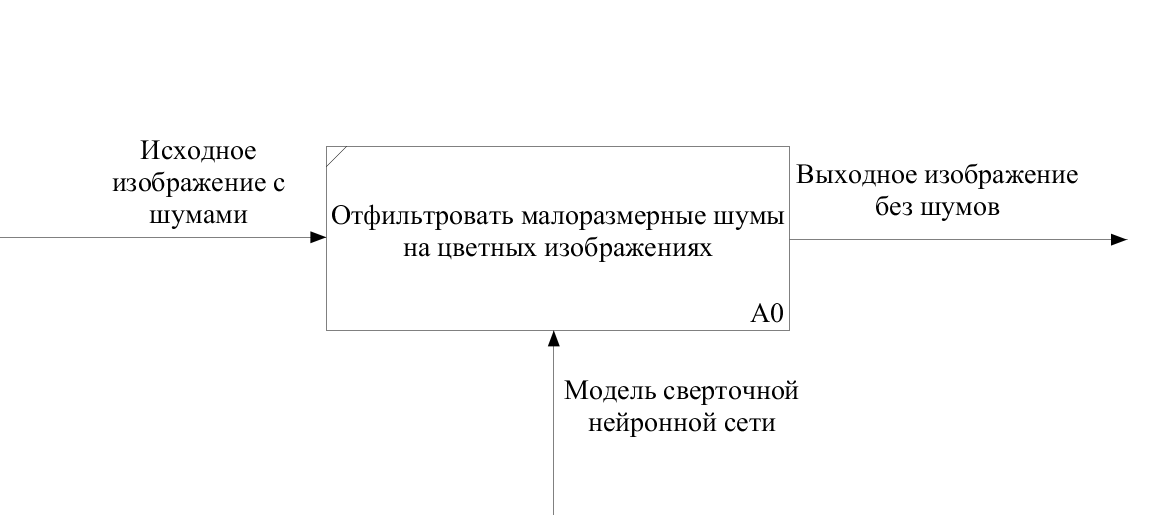
\includegraphics[scale = 0.5]{inc/analysis/01_A0.png}
	\caption{IDEF0--диаграмма нулевого уровня}
	\label{fig:idef0_0}	
\end{figure}

\section{Выводы}

В данном разделе был проведен анализ предметной области: были рассмотрены общие сведения о построении изображений, виды помех, которые могут возникать. Были рассмотрены алгоритмы нейронных сетей в следующих аспектах:
\begin{itemize}
    \item общие принципы работы нейронных сетей;
    \item различные функции активации и функции потерь;
    \item особенности обучения нейронных сетей, метод обратного распространения ошибки, а также критерии выбора данных для обучения;
    \item виды нейронных сетей.
\end{itemize}

В результате анализа были составлены сравнительная таблица методов устранения помех, сравнительная таблица видов нейронных сетей и сравнительная таблица организации архитектуры сверточных нейронных сетей.

Была выполнена формализация задачи в виде IDEF0--диаграммы.